% !TEX root = ../my-thesis.tex
%
\chapter{Future Perspectives: Active Learning}
\label{sec:al}

\cleanchapterquote{Qual è 'l geomètra che tutto s'affige; per misurar lo cerchio, e non ritrova; pensando, quel principio ond'elli indige. Tal era io a quella vista nova: 
veder voleva come si convenne; l'imago al cerchio e come vi s'indova. }{Dante Alighieri}{(Italian poet, 1265-1321)}

\section{Active Learning for piecewise surrogate models}
\label{sec:al:active_learning_piecewise}

Active learning is a powerful technique that can be used to improve the precision of our surrogate model by selectively adding new training points to the nDoE $\data$ where it is most needed. In this thesis, we have already touched upon active learning in \S\ref{sec:surr}, where we developed an active learning strategy for the emulator of the CMP hyperparameters.  

\smallskip
In that context, we were mostly interested in improving the precision of the surrogate model with respect to an unknown measure $\mathbb{P}(\dd \bx)$, which corresponded to a posterior distribution. A lot of effort was put into developing an iterative sampling strategy that could efficiently explore the posterior distribution and used an active learning strategy, proportional to the predictive variance of the surrogate model, to select new training points. Such a strategy originally comes the field of Optimal Experimental Design (OED)~\cite{kiefer1959,kiefer1960}, and put into a procedural form by~\cite{fedorov1972}. Its application and success in the context of GPR is due to~\cite{mackay1992}. Since then, variance based strategies have been widely used in a variety of applications, see~\cite{chen2026,tebbe2024} for a few examples. 

\smallskip
Variance-based strategies are also popular in the context of piecewise surrogate models, as they can be used to identify regions of the input space $\Omega$ where the surrogate model is most uncertain and where new training points would be most beneficial. A lot of work has been done in the context of GP regression, and practitioners use the predictive variance of the mixture reconstruction, Eq.~\eqref{eq:sota_2:mixture_reconstruction}, to guide the active learning process~\cite{riis2023, park2025}. The predictive variance of the mixture reconstruction can be computed using the law of total variance, 

\begin{equation}
    \mathbb{V}_{\hat{f}}[\hat{f}(\bx)] = \sum_{l=1}^L \mathbb{P}(\bx \in \Omega_l) \left( \mathbb{V}_{\hat{f}_l}[\hat{f}_l(\bx)] + (\mathbb{E}_{\hat{f}_l}[\hat{f}_l(\bx)] - \mathbb{E}_{\hat{f}}[\hat{f}(\bx)])^2 \right) \;.
    \label{eq:sota_2:mixture_var}
\end{equation}

Notice that the Eq.~\eqref{eq:sota_2:mixture_var} contains two terms: the first term is the weighted average of the variances of the local surrogate models $\mathbb{V}_{\hat{f}_l}[\hat{f}_l]$, and the second term is the weighted average of the squared differences between the means of the local surrogate models $\mathbb{E}_{\hat{f}_l}[\hat{f}_l]$ and the mean of the overall surrogate model $\mathbb{E}_{\hat{f}}[\hat{f}]$. This second term captures the uncertainty due to the classification task, and it is often referred to as the \textit{model uncertainty}. 

\smallskip
While variance-based strategies are very effective, they are primitive and can fail in some cases. Consider the case in which the function $f$ has a jump; the predictive variance of the surrogate model will always be high near the jump. As an example, consider the function $f(x) = (-1)^{\mathbb{I}(x < 0)}\, \frac{1}{10} \sin 2 \pi x $ defined on the interval $[-1,1]$. This function has a jump at $x=0$, and it is almost constant on both sides of the jump. 

\begin{figure}[htbp]
    \centering
    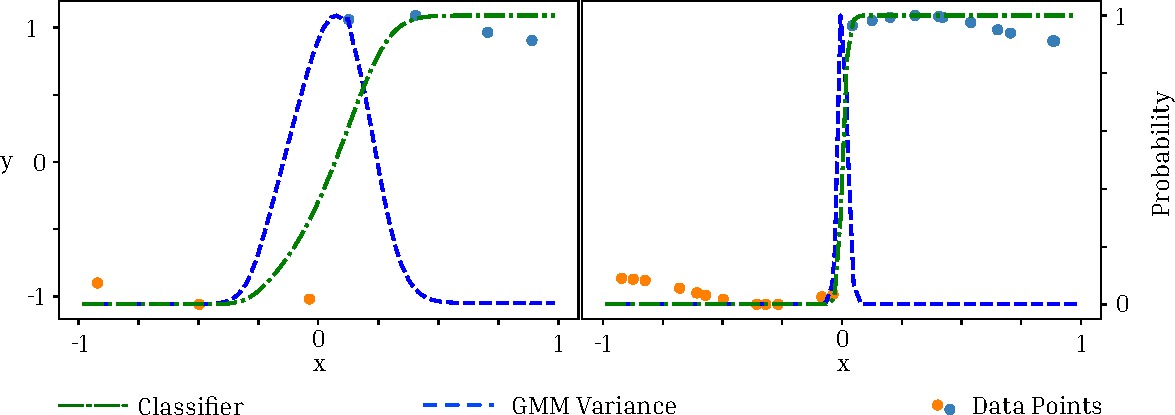
\includegraphics[width=\textwidth]{figures/sota_2/p_var.pdf}
    \caption{Schematic representation of the failure of variance-based active learning strategies in the presence of a jump.}
    \label{fig:sota_2:active_learning}
\end{figure}

Fig.~\ref{fig:sota_2:active_learning} provides a schematic representation of the failure of variance-based active learning strategies in the presence of a jump. Eq.~\eqref{eq:sota_2:mixture_var} is reported (normalized to be between 0 and 1) as a blue dashed line while the green line corresponds to the classifier probability $\mathbb{P}(\bx \in \Omega_1)$, which is close to 0 for $x < 0$ and close to 1 for $x > 0$. As we can see, increasing the size of the training set $\data$ pushes the acquisition function to be more and more concentrated near the jump, which is not ideal as adding a point near the jump would not lead to a significant improvement of the surrogate model.

\smallskip
These issues call for the development of more sophisticated active learning strategies. For standard GPs (without clustering), in~\cite{cohn1996}, the authors propose to use an active learning strategy based on the expected reduction in the predictive variance of the surrogate model, which is often referred to as \textit{active learning Cohn} (ALC). Similarly to variance-based strategies, ALC recognizes that the predictive variance is a good proxy for the predictive error (which ultimately comes from the bias-variance decomposition of the error), but selects the new training point based on how much it would reduce the predictive variance globally. Formally, the ALC acquisition function is defined as,


\begin{equation}
    \alpha_{\text{ALC}}(\bx^\prime) = \int_{\Omega} \left( \mathbb{V}_{\hat{f} \mid \data \cup \{\bx^\prime\}}(\bx) - \mathbb{V}_{\hat{f} \mid \data}(\bx) \right) \mathbb{P}(\dd \bx) \;.
\end{equation}

Notice that for GP regression, the integrand quantity admits a closed-form solution, as we discussed in \S\ref{sec:ntools:evr}. Furthermore, the ALC also elegantly solves the problem of batch selection. This problem has not been addressed yet in the context of piecewise surrogate models and all the works that we are aware add one point at a time. Notice that adding one point at a time can not only be inefficient but also impractical in all cases in which the solver is run in parallel and computes more than one point at a time. ALC, on the other hand, can be adjusted to select a batch of points by iteratively adjusting the acquisition function to account for the points that have already been selected, as we did in \S\ref{sec:surr} to improve the variance based strategy.

\smallskip
While for a single global GP a closed-form expression for the global variance reduction exists, the same is not true for a piecewise GP. Hence, our effort in the next chapter will be to derive such an expression.

\section{Closed form ALC criterion for piecewise GP}
\label{sec:al:alc}

To compute the Expected Variance Reduction (EVR) at a target point $\bx$ given a candidate sample at $\bx_*$, we leverage the Law of Total Variance. Let $y_*$ be the virtual observation at $\bx_*$ with noise variance $\sigma_\varepsilon^2$, and let $c_* \in \{1, \dots, L\}$ be the latent domain assignment for the new point. 

The current predictive variance $\mathbb{V}_{\hat{f}}[\hat{f}(\bx)]$ can be decomposed into the expectation of the posterior variance and the variance of the posterior mean:
\begin{equation}
    \mathbb{V}_{\hat{f}}[\hat{f}(\bx)] = \mathbb{E}_{y_*, c_*} \left[ \mathbb{V}_{\hat{f}}[\hat{f}(\bx) \mid y_*, c_*] \right] + \mathbb{V}_{y_*, c_*} \left[ \mathbb{E}_{\hat{f}}[\hat{f}(\bx) \mid y_*, c_*] \right] \;.
\end{equation}

The EVR is defined as the difference between the current variance and the expected posterior variance. This corresponds exactly to the second term:
\begin{equation}
    \text{EVR}(\bx; \bx_*) = \mathbb{V}_{y_*, c_*} \left[ \mathbb{E}_{\hat{f}}[\hat{f}(\bx) \mid y_*, c_*] \right] \;.
    \label{eq:evr_definition}
\end{equation}

Under the standard Active Learning assumption, the classification probabilities $\mathbb{P}(\bx \in \Omega_l)$ remain fixed during the look-ahead step. If the candidate point is assigned to domain l (i.e., $c_* = l$), only the l-th expert is updated. The posterior mixture mean becomes:
\begin{equation}
    \mathbb{E}_{\hat{f}}[\hat{f}(\bx) \mid y_*, c_*=l] = \mathbb{E}_{\hat{f}}[\hat{f}(\bx)] + \mathbb{P}(\bx \in \Omega_l) \frac{\mathbb{C}\text{ov}_{\hat{f}_l}[\hat{f}_l(\bx), \hat{f}_l(\bx_*)]}{\mathbb{V}_{\hat{f}_l}[\hat{f}_l(\bx_*)] + \sigma_\varepsilon^2} \left( y_* - \mathbb{E}_{\hat{f}_l}[\hat{f}_l(\bx_*)] \right) \;.
\end{equation}

To find the variance of this updated mean over the joint distribution of $y_*$ and $c_*$, we first evaluate the conditional expectation given the assignment $c_*=l$. Since $y_* \mid c_*=l \sim \mathcal{N}(\mathbb{E}_{\hat{f}_l}[\hat{f}_l(\bx_*)], \mathbb{V}_{\hat{f}_l}[\hat{f}_l(\bx_*)] + \sigma_\varepsilon^2)$, the expected squared difference from the prior mean is:
\begin{align}
    \mathbb{E}_{y_* \mid c_*=l} \left[ \left( \mathbb{E}_{\hat{f}}[\hat{f}(\bx) \mid y_*, c_*=l] - \mathbb{E}_{\hat{f}}[\hat{f}(\bx)] \right)^2 \right] 
    &= \mathbb{P}(\bx \in \Omega_l)^2 \frac{\mathbb{C}\text{ov}_{\hat{f}_l}[\hat{f}_l(\bx), \hat{f}_l(\bx_*)]^2}{\left( \mathbb{V}_{\hat{f}_l}[\hat{f}_l(\bx_*)] + \sigma_\varepsilon^2 \right)^2} \mathbb{V}_{y_* \mid c_*=l}[y_*] \nonumber \\
    &= \mathbb{P}(\bx \in \Omega_l)^2 \frac{\mathbb{C}\text{ov}_{\hat{f}_l}[\hat{f}_l(\bx), \hat{f}_l(\bx_*)]^2}{\mathbb{V}_{\hat{f}_l}[\hat{f}_l(\bx_*)] + \sigma_\varepsilon^2} \;.
\end{align}

Finally, we take the expectation over the discrete domain assignment $c_*$, where the probability of the candidate point belonging to domain l is $\mathbb{P}(c_* = l) = \mathbb{P}(\bx_* \in \Omega_l)$. This yields the final analytical expression for the Expected Variance Reduction:
\begin{equation}
    \text{EVR}(\bx; \bx_*) = \sum_{l=1}^L \mathbb{P}(\bx_* \in \Omega_l) \mathbb{P}(\bx \in \Omega_l)^2 \frac{\mathbb{C}\text{ov}_{\hat{f}_l}[\hat{f}_l(\bx), \hat{f}_l(\bx_*)]^2}{\mathbb{V}_{\hat{f}_l}[\hat{f}_l(\bx_*)] + \sigma_\varepsilon^2} \;.
    \label{eq:mixture_evr_final}
\end{equation}
